\documentclass[12pt]{ut-thesis}
\usepackage{xcolor}
\usepackage{graphicx}
\usepackage{lscape}
\usepackage{amssymb}
\usepackage{amsmath}
\usepackage{cite}


\degree{Doctor of Philosophy}
\department{Molecular Genetics}
\gradyear{2017}
\author{Jochen Weile}
\title{An atlas of variant effects in human disease genes}

\newcommand{\gene}[1]{\textit{#1}}
\newcommand{\species}[1]{\textit{#1}}
\newcommand\todo[1]{\texttt{\textcolor{red}{\textbf{TODO:} #1}}}
\newcommand{\celsius}{$^{\circ}$C}
\newcommand{\etal}{\textit{et~al.}}

%% List only down to subsections in the table of contents;
%% 0=chapter, 1=section, 2=subsection, 3=subsubsection, etc.
\setcounter{tocdepth}{2}

%% Make each page fill up the entire page.
\flushbottom


%%%%%%%%%%%%      MAIN  DOCUMENT      %%%%%%%%%%%%

\begin{document}


\begin{preliminary}

\maketitle

%% There should be NOTHING between the title page and abstract.
%% However, if your document is two-sided and you want the abstract
%% _not_ to appear on the back of the title page, then uncomment the
%% following line.
%\cleardoublepage

\begin{abstract}
%% (At most 350 words for Ph.D.)

Although we now routinely sequence human genomes, we cannot yet confidently identify functional variants. Here a deep mutational scanning framework is developed that combines random codon-mutagenesis and multiplexed functional variation assays with computational imputation and regularization to yield look-up tables for human missense variants. The framework is applied to five proteins corresponding to seven human genes: UBE2I (encoding SUMO E2 conjugase), SUMO1 (small ubiquitin-like modifier), NCS1 (neuronal calcium sensor 1), TPK1 (thiamin pyrophosphokinase), and CALM1/2/3 (three genes encoding the protein calmodulin). The resulting functional impact scores correspond to known protein features, and serve to confidently identify pathogenic variation. %Analysis of large-scale phenotypic screens suggests that assays potentially amenable to deep mutational scanning are already available for 57\% of human disease genes.
\end{abstract}

%\begin{dedication}

%\end{dedication}

\begin{acknowledgements}
The author gratefully acknowledges funding by the National Institutes of Health, the Canadian Excellence Research Chair, the Canadian Center for Advanced Research and the Ontario Ministry of Research and Innovation. The author would also like to thank Fritz Roth, Atina Cote, Jennifer Knapp, Song Sun, Marta Verby, Yingzhou Wu, Cassandra Wong, Fan Yang, Carles Pons, Natascha van Lieshout, Anjali Gopal,  Guihong Tan, Joseph Mellor, Brenda Andrews, Charles Boone, Nidhi Sahni, Marc Vidal, and David Hill for their collaboration.
\end{acknowledgements}

\tableofcontents

%\listoftables

%\listoffigures

%% You can add commands here to generate any other material that belongs
%% in the head matter (for example, List of Plates, Index of Symbols, or
%% List of Appendices).

%% End of the preliminary sections: reset page style and numbering.
\end{preliminary}


%% Introduction: Length: 25-30 pages.
%%  * Relevant background, 
%%  * Outline of state of knowledge, 
%%  * emphasize outstanding questions 

\chapter{Introduction}

Given the constantly improving cost and speed of genome sequencing, it is reasonable to expect that within the coming decades personal genomes will be known for a substantial part of the global populace. Unfortunately, our limited ability to interpret the variation found within them stands in stark contrast with this development. Even when limiting ourselves to mutations in coding regions of the genome, the effects of most missense variants are not known. While a number of computational approaches exist to make predictions as the effects of coding variants, they are currently not reliable enough for clinical use. Laboratory assays by comparison produce more trustworthy results, but until recently did not scale to the space of all possible mutations. The development of Deep mutational scanning\cite{Fowler2010} has now made this endeavour possible. In the following sections, each of these issues will be discussed in detail.

\section{The Genotype-Phenotype Problem}

Linking genotype to phenotype is a very difficult problem. The part of the human genome we understand best are protein-coding genes, yet they only constitute a minuscule fraction the whole. Impacts of mutations in other functional elements such as introns, untranslated regions of genes, or regulatory sequences, are more difficult to assay, not to mention the vast stretches of intragenic space. While one might expect the latter to not bear functional significance a priori, its importance is nonetheless highlighted by the the fact that a large number of loci identified as correlated with diseases in genome-wide association studies (GWAS) are found within these regions\cite{TODO}.
But even for protein-coding sequences the problem is far from simple. Alleles that behave according to the Mendelian model are the exception. Most phenotypes are complex, i.e. emerge through the interplay of many different genetic or environmental factors. Conversely, many genes are also pleiotropic, i.e. they are involved more than one mechanism. Thus, a mutation found in one person may not have the same effect as in another---a phenomenon called incomplete penetrance. Similarly, two different mutations within the same coding sequence need not have the same effect either. Depending on how the translated protein is affected (catastrophic folding failure, alteration of a molecular interaction interface or active site, or a subtle change on an unused surface) the effects may differ in severity or in rare cases even in the emergence of new behaviours.

Given the much greater difficulty of interpreting non-coding regions, clinical applications have so far largely concentrated on protein-coding genes. Sequencing panels for known disease-associated genes and even whole-exome sequencing (WES) are widely commercially available. A number of different standards for classifying mutations with respect to their potential health impacts have been proposed. Most prominently, the American College of Medical Genetics and Genomics (ACMG) standard\cite{?}. It defines categories stretching from ``pathogenic'' via ``variant of uncertain significance'' (VUS) to ``benign''. Even though the mutational landscape for a handful of genes, such as \gene{BRCA1} are explored better than others due to their high monetization potential\cite{BRCA_Clinic}, the vast majority of clinical variants are currently classified as VUS. For example, over 98\% of missense variants for a gene panel assessing germline cancer risk variants~\cite{Maxwell2016} have been discarded as VUS. Not only can these uncertainties unduly burden patients with unnecessary anxiety, they also call into question the value of sequencing in the clinic if the majority of findings are not actionable. With increasing use of WES, this problem is only going to get worse. According to  the 1000 Genomes Project data, every person carries 100-400 missense variants that are so rare that they have likely never been seen before in the clinic~\cite{1000genomes}. In the absence of previous observations they would automatically be added to long list of VUS.

\section{\textit{In silico} approaches to variant function assessment}

A number of algorithms exist that offer predictions as to the deleteriousness of mutations, the most prominent ones being PolyPhen-2\cite{Polyphen}, SIFT\cite{SIFT} and PROVEAN\cite{PROVEAN}. PolyPhen-2 uses a machine learning method using evolutionary conservation and protein structural features. It uses a set of previously reported pathogenic alleles as a positive training set and differences between human genes and their mammalian homologues as a negative training set. SIFT (Sorting Intolerant From Tolerant) by contrast only uses evolutionary conservation. The tool uses multiple sequence alignments to calculate position-specific score matrices for each gene which are then normalized and transformed into probability values. PROVEAN (PROtein Variation Effect ANalyzer) similarly only takes into account sequence alignments. However, rather than just computing a position-specific score, PROVEAN calculates the difference in alignment quality between using the wildtype or variant sequence against clusters of homologous sequences. The average distance is then interpreted as indicative of the deleteriousness of the variant. 

While the three tools succeed in making good predictions, their reliability is unfortunately still not high enough to serve as a basis of clinical decision making. Song Sun recently performed an independent comparison of these tools on a set of well established disease-causing variants as well as rare polymorphisms with no known disease association\cite{SunExtendedSet}. A high precision (the fraction of correct classifications out of all positive classifications) can be considered especially important when considering taking clinical action based on a prediction. When compared at a minimum precision level of 90\%, PolyPhen-2 and PROVEAN only reach a sensitivity of 19\% and 21\% , respectively (where sensitivity is defined as the fraction of correct classifications out of all real existing disease variants). SIFT was not even capable of achieving 90\% precision at any score threshold.

\section{Functional Complementation}

\section{Binary Protein-Protein interactions and Yeast-2-Hybrid}

\section{Deep Mutational Scanning}

\section{Edgotyping}

\section{Background: The Sumoylation Pathway}



\chapter[High-fidelity and comprehensive DMS framework]{A framework for comprehensive and high-fidelity Deep Mutational Scanning}

\section{Introduction}

Within coming decades, millions of people will have their genome sequenced. Unfortunately, we have limited ability to interpret personal genomes, each carrying 100-400 rare missense variants1 of which many must currently be classified as “variants of uncertain significance”. For example, gene panel sequencing aimed at identifying germline cancer risk variants in families yielded VUS for the majority of missense variants2.  While functional variants can be predicted via computational tools such as PolyPhen-23 and PROVEAN4, these methods can confidently detect only one third as many disease variants as are detectable by experimental assays5. Unfortunately, experimental assays are either unavailable or economically inviable for most human disease genes. The development of Deep Mutational Scanning (DMS)6,7 is making it possible to produce maps that predict the functional impact of a large fraction of substitutions for at least a subset of residue positions. Recently, Starita and colleagues carried out a DMS screen for the critical RING domain of BRCA18. Despite this progress, no experimental sequence-function map has yet demonstrated high-accuracy scoring of the functional impact of all possible substitutions for any full length protein (see Supplementary Table S1). Thus, the goal of complete, highly accurate DMS maps for full-length proteins remains undemonstrated.

Functional complementation can measure the ability of a mutant human protein to rescue the loss of the wild type enzyme (or its ortholog in the case of trans-species complementation)9,10. We have previously found that cell-based functional complementation assays facilitated highly accurate identification of disease variation across a diverse collection of human disease genes5. 

Here we describe a modular DMS framework to generate maps of variant function. The framework employs a novel mutagenesis strategy, functional complementation, two alternative sequencing-based selection screens, and a machine learning strategy that completes the map via imputation and regularization. We first evaluate our framework on the SUMO E2 conjugase UBE2I.

\section{Results}

To carry out deep mutational scans of protein sequences yielding comprehensive atlases of sequence-function relationships, we found it useful to organize the process into six stages (see Figure 1A): 1) mutagenesis; 2) generation of a clone library; 3) selection for clones encoding a functional protein; 4) read-out of the selection results and analysis to produce an initial sequence-function map; 5) computational analysis to impute missing values; and 6) computational analysis to refine measured values based on imputation models. This framework incorporates previously-described deep mutational scanning concepts as well as new experimental components (e.g., our saturation codon mutagenesis strategy) and analytic methods.  The last two stages enabling a complete and accurate DMS map have not been applied in any published DMS study.

We first describe a variant of the framework called DMS-BarSeq and apply it to the human SUMO conjugase UBE2I, exhaustively measuring the ability of protein variants to function and to physically interact with protein partners.  Next, we describe a more efficient DMS-TileSeq variant of the framework, and apply this to UBE2I.  Having combined these maps, we computationally infer missing data points and refine map quality.

\subsection{A barcode-based Deep Mutational Scanning strategy}

As an initial test of the overall framework, we first aimed to generate a map of functional missnse variation for UBE2I. For Stage 1 of the DMS framework—mutagenesis—we wished to achieve a relatively even representation of all possible single amino acid substitutions.  Furthermore, we wished to allow multiple mutations per clone, both because this could allow for greater mutational coverage for any given library size, and because it would offer an opportunity to discover intragenic epistatic relationships between variants.  To fulfill these requirements, we developed a mutagenesis protocol (Precision Oligo-Pool based Code Alteration or POPCode) which generates random codon replacements. POPCode scales up a previously-described technique11 in which oligonucleotides carrying a central 3-base degenerate region are hybridized to a uracil-containing wild-type DNA template, with completion of the mutant strand via non-displacing DNA polymerase extension and ligation, followed by degradation of the wild-type template (see Supplementary Methods).  To accomplish mutagenesis across the entire coding region, we designed a tiled collection of oligos (one per codon) and applied POPCode to generate a codon-mutagenized amplicon library for UBE2I.  In parallel, we carried out PCR with oxidized nucleotides 12 to enable deeper representation of amino acid changes achievable from single-nucleotide changes.

For Stage 2 of the framework—generation of a clone library—we employed an en masse recombinational cloning strategy to generate a Gateway Entry vector library of UBE2I variants (see Online Methods). This library was then transferred via en masse recombinational subcloning into a pool of randomly-barcoded plasmids enabling expression of UBE2I variants in yeast. The full-length sequence and barcode of each clone was established using a novel sequencing method called kiloSEQ which combines plate-position-specific index sequences with Illumina sequencing to carry out full-length sequencing for thousands of samples (see Online Methods). Based on sequence information, we retained clones that carried at least one amino acid substitution to generate a final library comprised of 6,553 UBE2I variants, covering different combinations of 1,848 (61\% of all possible) unique amino acid changes. Variant plasmids were pooled, together with empty vector and wild type control plasmids (see Online Methods).

For Stage 3, the selection of clones encoding a functional protein, we employed a previously described S. cerevisiae functional complementation assay5,13. This assay is based a yeast strain carrying a temperature sensitive (ts) allele of the UBE2I orthologue UBC9, and on the observation that human UBE2I rescues growth at an otherwise lethal elevated temperature.  Despite a billion years of divergence, yeast functional complementation assays of human disease genes can accurately discriminate pathogenic from non-pathogenic variants5,13.  The plasmid library from Stage 3 was introduced into the appropriate ts strain by en-masse transformation. Pools were then grown over a period of 48 hours at the permissive (25°C) and selective (37°C) temperatures, respectively (see Online Methods).

To read out the results of the selection (Stage 4), barcodes were sequenced at multiple timepoints to enable reconstruction of individual growth curves and normalized fitness quantification for each of the 6,553 strains. Functional complementation scores were calibrated so that a value of 0 corresponds to the mean fitness of the empty-vector control and a value of 1 corresponds to the average of wild type controls (see Online Methods).
To assess the quality of complementation scores before further refinement in Stages 5 and 6, we first examined reproducibility of scores between technical replicates (Figure 1B, top panel), and biological replicates (different clones carrying the same mutation; Figure 1B, bottom panel).  In each case the scores were reproducible (Pearson’s R of 0.97 and 0.78, respectively).   To further examine score quality, we carried out semi-quantitative manual complementation spotting assays for a subset of mutants that spanned the range of fitness scores (see Supplementary Methods). Complementation scores from deep mutational scanning correlated well with these small-scale tests. Indeed, agreement between the large-scale and manual scores was about the same as agreement between internal replicates of the large-scale scores (Figure 1B,C). 

As a further ‘sanity check’, we next examined evolutionary conservation and common predictors of deleteriousness, such as PolyPhen-23 and PROVEAN4.  Although these do not perfectly predict the functionality of amino acid changes5 —and may be particularly ill-suited for assessing amino acid changes that require multiple nucleotide substitutions in a given codon—they should nonetheless correlate with functionality.  Indeed, DMS-BarSeq fitness scores were significantly correlated with evolutionary conservation and PolyPhen-2 and PROVEAN scores (Figure 1D top panel, Supplementary Figure S1). Finally, we confirmed that, as expected, amino acid residues on the protein surface are more tolerant to mutation than those in the protein core or within interaction interfaces (Figure 1D, bottom panel).  Taken together, these observations support the biological relevance of the DMS-BarSeq approach.


\subsubsection{POPCode: A Precision Oligo Pool Codon alteration mutagenesis method}

This method scales up a previously described method developed by Seyfang et al.11. To achieve complete wide coverage over the complete spectrum of possible amino acid changes we design oligonucleotides centering on each codon in the Open Reading Frame (ORF) of interest and replacing the target with a NNK degeneracy code. This has been previously demonstrated to allow all amino acid changes while reducing the chance of generating stop codons36 . 

When finding a set of suitable oligonucleotide sequences, two important criteria need to be considered; 
1) The melting temperature across the complete set is as uniform as possible as this will ensure a more even mutation rate across the ORF sequence; 2) the degenerate codon sequence should be located as close to the center of the oligo as permissible given the first criterium. To simplify the process of choosing an appropriate set of oligos based on these criteria I developed a web tool that can be used to calculate the optimal solution to the given problem. The tool merely requires the sequence of the target ORF and flanking vector sequences, a desired average oligo length and a maximum offset parameter. The offset parameter determines how many bases can be maximally added or removed from each side of a given oligo to optimize its melting temperature. 

In the next step, the ORF sequence is PCR amplified in the presence of dUTP to generate uracil-doped template for the mutagenesis reaction. Oligonucleotide pools were then hybridized with the template. Gaps between hybridizations were filled and sealed with the non-strand-displacing Sulpholobus Polymerase IV. Following cleanup, the uracil-doped template was incapacitated using Uracil-DNA-Glycosylase (UDG). The mutagenesis product was then amplified with primers that added attB sites to allow Gateway BP cloning into entry vectors.

\subsubsection{KiloSEQ: A highly multiplexed amiplicon sequencing method}

To establish the identity of each plasmid barcode and its associated set of mutations in the target ORF we used kiloSEQ, which was developed in collaboration with SeqWell Inc., Boston. The ORF and barcode locus are in close proximity to each other on the plasmid. Thus we can amplify a smaller segment of the plasmid containing both for sequencing. This is done using a hydrocycler, allowing for thousands of PCR reactions to be performed in parallel. The primers used in these reactions contain well-specific tags allowing each well on each plate to be uniquely identified. Amplicons can then be plate-wise pools. In the next step, Nextera tagmentation using Tn5 transposase is used to break the amplicons into shotgun fragments and ligate them to Illumina sequencing linkers. We then re-amplify those fragments that contain the original well-specific tags. The resulting library is now ready for paired-end sequencing using Illumina NextSEQ 500, where each plate can be tagged with a unique Nextera sequence index. In each pair of reads, one read will contain the well tag and the barcode locus, whereas the other will contain a fragment of the mutant ORF.

We developed a sequence analysis pipeline to perform demultiplexing, barcode identification and genotyping. The pipeline source code is available upon request. In the first step Illumina bcl2fastq is used to demultiplex the reads at the plate level using the custom Nextera indices. The resulting FASTQ files are then further demultiplexed using the well-tags in a highly parallel fashion. This results in a folder structure containing tens of thousands of individual fastq files sorted by plate and well coordinate. These are then further processed in parallel to identify barcodes. Due to the limitations of the Biomatrix robot, wells can sometimes contain more than one clone. Thus barcode sequences are extracted from each read and then clustered by edit distance to determine the set of barcodes in each well. The associated paired reads for each barcodes are then further split by barcode. Each barcode-specific set of ORF reads can then be analyzed with respect to mutations. Bowtie2 software is used to align reads to the ORF template, PCR duplicates are removed and nucleotide variants called using samtools pileup. Due to the effects of the kiloSEQ PCR steps on read coverage, identification of longer indels is not straightforward. A solution was found by extracting depth of coverage tracks for each clone and normalizing them with respect to average positional coverage across each 384-well plate. Then, an edge-detection algorithm is used to find sudden increases or decreases within the normalized coverage, indicating the presence of insertions or deletions.

After successful genotyping with kiloseq, we determined the subset of clones that (i) contained a minimum of one missense mutation, (ii) did not contain any insertions or deletions, (iii) did not contain mutations outside of the ORF, (iii) had unique barcodes, (iv) had sufficient read coverage during kiloSEQ to allow for confident genotyping. Using the Biomatrix robot, we re-arrayed this filtered subset of clones into a condensed final library of 40 plates.

\subsubsection{A barcoded-based functional map of UBE2I}

\subsection{A complete functional map of UBE2I}

\subsubsection{An alternative strategy for DMS via tiled regional sequencing}

While the DMS-BarSeq approach has many advantages (see Discussion), its performance comes at the cost of producing and maintaining an arrayed clone library, and of determining the full-length sequence of each coding region and barcode for each clone. We therefore investigated an alternative approach called DMS-TileSeq: Instead of tracking the fitness of each individual clone, we carried out en masse measurements of the frequency of each variant in the pool before and after selection, by deep sequencing.  Sequencing was carried out for a set of short amplicon tiles that collectively encompass the complete coding region.  In this way, we can discern the impact of each mutation by observing the impact of selection on the abundance of clones carrying this mutation.

In terms of mutagenesis (Stage 1), DMS-TileSeq is identical to DMS-BarSeq.  Given the mutagenized amplicon library, the cloning step (Stage 2) was carried out by en masse recombinational subcloning into complementation vectors (thus skipping the step of arraying and sequencing individual clones).  This plasmid pool was next transformed en masse into the ubc9-ts strain appropriate for assessing the complementation ability of UBE2I variants. As with DMS-BarSeq, DMS-TileSeq employs pooled strains grown competitively (Stage 3) at the permissive and selective temperatures. However, instead of using barcode sequencing to determine the fitness associated with individual stains, we directly sequence the coding region from the clone population to determine the frequency of each variant in each pool (before and after selection). To overcome the problem of distinguishing mutations from sequencing errors, we divide the coding region into tiles such that each individual template molecule can be completely sequenced on both strands.  By requiring that each variant be seen on both strands, the incidence of base-calling errors can be substantially reduced6.  DMS-TileSeq requires that the library be sufficiently complex to ensure that the effect of a mutation is determined from enough clones and over enough genetic backgrounds (where there are multiple variants per clone) to be reproducible (see Online Methods).

To validate the reliability of DMS-TileSeq, we first applied it to UBE2I and compared the results with those obtained using DMS-BarSeq. Correlation between DMS-TileSeq and DMS-BarSeq was comparable to the correlation observed between biological replicates of DMS-BarSeq (Supplementary Figure 2), suggesting that reproducibility of DMS-TileSeq is at least comparable to that of DMS-BarSeq. DMS-TileSeq and DMS-BarSeq showed comparable agreement with complementation scores from manual assays (Supplementary Figure 3).  Thus, DMS-TileSeq avoids the substantial cost of arraying and sequencing thousands of individual clones, while performing on par with DMS-BarSeq in terms of reliability of the functional complementation scores it produces.


\subsubsection{Imputation and regularization of missing or less accurate data}

Having performed two independent deep mutational scans of UBE2I using functional complementation assays, we wished to integrate both results into a single comprehensive high-quality map. To accomplish this, we first combined the results of each screening approach into a joint map.  This required bringing the maps onto the same scale. Using a regression-based transformation function, we transformed the DMS-TileSeq scores to the more intuitive scale of DMS-BarSeq (where 0 corresponds to the typical score of a null mutant and 1 corresponds to the typical score of a wildtype control). We then combined scores from the two methods, giving greater weight to more confident measurements (see Online Methods).

As is the case for all previously published DMS maps, our combined map contained some entries that were poorly measured or missing (e.g., because these substitutions were underrepresented in the input clone library). To fill in the gaps, we trained a machine learning model to impute missing data (Stage 5 of our framework). Specifically, we trained a random forest regression model on a set of biochemical and structural features, as well as features intrinsic to our dataset (for example, the average score of well-measured substitutions at a given position). This procedure also allowed incorporation of information from clones in DMS-BarSeq that had multiple mutations, through the use of two features: 1) the average score of all clones carrying the mutation of interest, and 2) the average corrected score from clones that carry the mutation of interest, where the correction makes use of a multiplicative fitness model to remove the fitness effect of other mutations present (see Supplementary Methods). We assessed performance of the imputation model using cross-validation and found that the root-mean squared deviation of imputed values is on par with measurement error in experimentally measured data (Supplementary Figure S3).

To improve the accuracy of entries for which the experimental measurements were least confident, we employed a regularization method (Stage 6 of the framework).  This was achieved by combining experimental measurements and imputed values, weighting by the estimated accuracy of each (see Methods). The complete refined functional map of UBE2I after imputation and regularization can be seen in Figure 2A. 

To evaluate the complete map, we applied manual functional complementation assays to a set of variants that were chosen to represent the full range of fitness scores.  DMS fitness scores corresponded closely with manual functional complementation assays (Supplementary Figure S4A), validating our framework.  To more specifically evaluate the imputation process, we selected a smaller test set of variants (again spanning the range of impact scores), and recalculated imputation scores after excluding variants in the test set from the training process.  Imputed scores not only corresponded closely with measured DMS scores, but also with the results of manual complementation assays (Supplementary Figure S4B).  Collectively, our framework yielded a comprehensive map covering all possible missense variants, with overall quality that was on par with the highest-quality measurements from either screen alone.


\subsection{Evaluation and validation of the UBE2I map}

\section{Methods}

\section{Discussion}




\chapter[Expanding the atlas of human disease variants]{Expanding the atlas of variant effects in human disease genes}

\section{Introduction}

Within coming decades, millions of people will have their genome sequenced. Unfortunately, we have limited ability to interpret personal genomes, each carrying 100-400 rare missense variants~\cite{the_1000_genomes_project_consortium_global_2015} of which many must currently be classified as Variants of Uncertain Significance (VUS). For example, gene panel sequencing aimed at identifying germline cancer risk variants in families yielded VUS for the majority of missense variants~\cite{maxwell_evaluation_2016}. While functional variants can be predicted via computational tools such as PolyPhen-2~\cite{adzhubei_predicting_2001} and PROVEAN~\cite{choi_predicting_2012}, these methods can confidently detect only one third as many disease variants as are detectable by experimental assays~\cite{sun_extended_2016}. Unfortunately, experimental assays are either unavailable or economically inviable for most human disease genes. 

Recent DMS studies have provided individual maps the critical RING domain of BRCA1~\cite{starita_massively_2015} associated with breast cancer risk, and the PPAR$\gamma$ protein associated with Mendelian lipodystrophy and increased risk of type 2 diabetes~\cite{majithia_prospective_2016}. Such maps can not only identify functionality of a clinical variant accurately, but also potentially do so in advance of that variant's first clinical presentation. 

In the previous chapter, we established a framework for comprehensive high-quality screening of the functional effects across all possible missense mutations in human genes. The functional complementation assay used in the assay allows for the generation of maps that not only represent the overall functional consequences of mutations, but also serves as a common basis to make maps more directly comparable. In addition, the statistical analysis and machine learning component we introduced supports allows for high overall map quality and completeness. Using this framework we have created a complete functional map for the SUMO E2 conjugase UBE2I. Here we create a map of a second member of the Sumoylation pathway, SUMO1. We examine both map in detail before discussing the interpretation of yeast complementation phenotypes in terms of humans. 

To demonstrate the value of our frameworks in terms of clinical interpretation of variants, we proceed to add a diverse set of six new disease gene maps to our atlas: TPK1 encoding Thiamin Pyrophosphokinase 1, NCS1 encoding Neuronal Calcium Sensor 1, as well as the paralogues CALM1, CALM2 and CALM3, which each encode the protein Calmodulin. We evaluate the maps in terms of pathogenicity prediction and VUS reclassification.

\section{Results}

% \todo{Outline the structure of the results section}

\subsection{Functional map of SUMO E2 recapitulates known biology and poses new questions}

% \todo{Quickly recap how maps for UBE2I and SUMO1 were made}

The DMS map of UBE2I produced in the previous chapter paints a comprehensive picture of variant effects on protein function (Figure~\ref{fig:ube2i-map}). Based on the map, several observations can be made. Consistent with the results of smaller-scale biochemical studies of the SUMO E2 conjugase\cite{bencsath_identification_2002,bernier-villamor_structural_2002}, the areas most sensitive to mutation are those proximal to the active site (particularly residues 81-88, 90, 92-96, and 127-130), and the N-terminal $\alpha$-helix which mediates four protein interactions including the critical interaction with the E1 SUMO-activating complex. Within the active site, particularly strong sensitivity to mutation can be observed at the Cystein residue at position 93. This is consistent with its central role in E2 function, as it forms a thioester bond with the SUMO C-terminus~\cite{bernier-villamor_structural_2002}.

An interesting feature of the map is the alternating tendency towards damaging and benign substitutions across positions 55-65. A comparison with solvent accessibility reveals this to be caused by alternating externally and internally-oriented residues, with the latter positions constrained to be hydrophobic. This alternating tendency is also reflected in evolutionary conservation across these positions. 

All protein-protein interaction interfaces previously captured in co-crystal show increased sensitivity to mutation when compared to other surface residues (Figure~\ref{fig:ube2i_interfaces}). When comparing individual protein interaction interfaces, the most substantial fitness defects are observed in those for the E1 activating complex binding interface and the covalent and noncovalent SUMO binding interfaces (Figure~\ref{fig:ube2i_interfaces}A). While the homodimerization interface also shows significant sensitivity, the effects are not as severe as those at the E1 interface (Figure~\ref{fig:ube2i_interfaces}B). This is consitent with the Alontaga and colleagues' hypothesis regarding its involvement in SUMO chaining~\cite{alontaga_rwd_2015}, as in yeast SUMO chain formation has so far only been observed to be involved in meiosis, which is not a mechanism vital to fitness in a complementation assay. Alontaga \etal also postulate however, that noncovalent SUMO binding is necessary for SUMO chain formation. In contrast to the homodimerization interface, the noncovalent SUMO binding interface shows a very strong sensitivity to mutation. This may be due to two different reasons: (i) there is a 27\% overlap between the interface for noncovalent SUMO binding interface and the interface for E1-E2 binding, which is among the most sensitive surfaces in UBE2I; and (ii) noncovalent SUMO binding also plays an important role as an adapter for many E3 proteins~\cite{cappadocia_structural_2015}.
%FIXME: Cappadocia: Structural basis for catalytic activation by the human ZNF451 SUMO E3 ligase


\begin{figure}[h!]
	\centering
	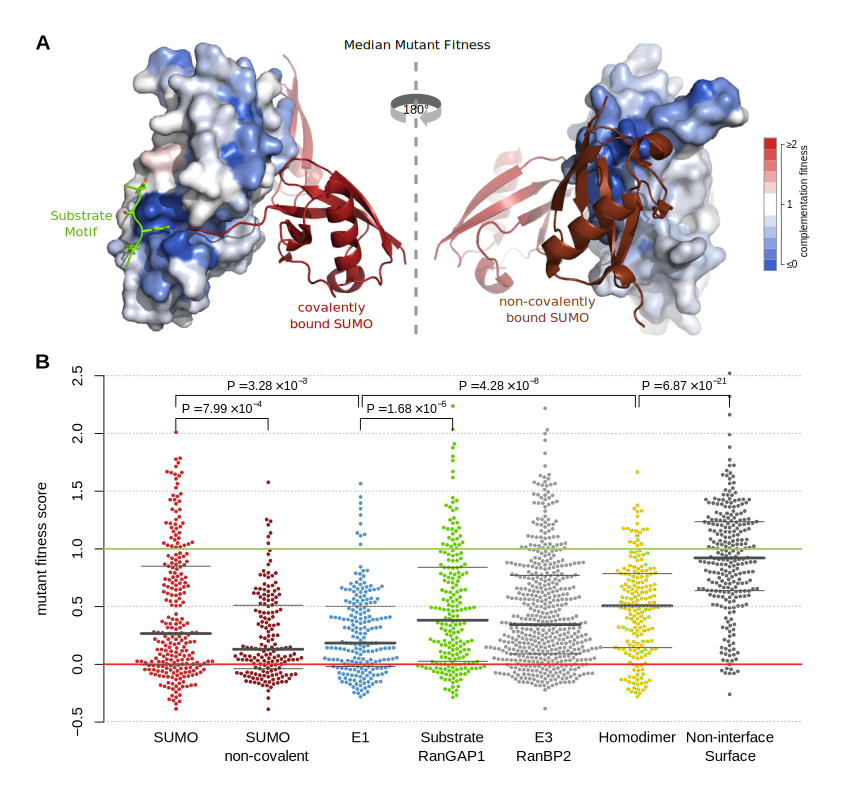
\includegraphics[width=\textwidth]{img/ube2i_interfaces.pdf}
	\caption{Complementation fitness of mutations at interaction interfaces. A) Median mutant fitness mapped to the crystal structure of UBE2I. The $\Psi$KXE substrate recognition motif is shown as green stick model, covalently and non-covalently bound SUMO are shown as crimson and brown cartoon model, respectively. B) Mutant fitness scores distributions for residues at different interaction interfaces. }
	\label{fig:ube2i_interfaces}
\end{figure}

Another interesting observation can be made with respect to a known phosphorylation site on the surface of UBE2I. Su and colleagues previously discovered that phosphorylation of Serine 71 via the Cyclin-dependent Kinase CDK1 results in sumoylation hyperactivity~\cite{su_phosphorylaton_2012}. Our map shows that substitutions with phosphomimetic residues at this position lead to hyperactive complementation, consistent with Su \etal.'s observations. Furthermore, other residues amenable to phosphorylation are also tolerated, while hydrophobic replacements are generally deleterious (Figure~\ref{fig:phosphosite}).
%FIXME: Su2012: Phosphorylation of Ubc9 by Cdk1 enhances SUMOylation activity

\begin{figure}
	\centering
	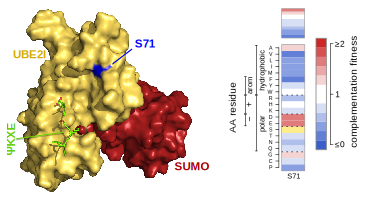
\includegraphics[width=\textwidth]{img/phosphosite.pdf}
	\caption{Phoshporylation site of UBE2I shows hyperactive complementation when mutated to phosphomimetic residues.}
	\label{fig:phosphosite}
\end{figure}


\subsubsection{Substrate specificity shifts and E2 hyperactivity}

Intriguingly, many sites show fitness that is better than wildtype (e.g., positions 74, 76, 88, 89, 91 and 98). Manual functional complementation spotting assays confirmed that complementation with these mutants allows greater growth than does the wild type human protein, but resemble more closely the growth at the permissive temperature for the \textit{ubc9-ts} strain (Figure~\ref{fig:hyperactive}A). One might be tempted to interpret these cases as reversions to residues present in the yeast protein. However, a comparison of fitness score distributions between changes to S. cerevisiae  residues and those occurring in the distant species \species{Dictyostelium~discoideum} (amoeba) or \species{Drosophila~melanogaster} (fly) showed no significant difference (Figure~\ref{fig:hyperactive}B). Recognizing that in this assay, human UBE2I must function with the yeast versions of other sumoylation pathway members, it stands to reason that some substitutions could be adaptive by improving compatibility with yeast interaction partners. A comparison with co-crystal structure data~\cite{gareau_determinants_2012} shows that many of the apparently-adaptive residues are located on the surface facing the general direction of the substrate, with some being in direct contact with the substrate's sumoylation motif (Figure~\ref{fig:hyperactive}C). This suggests a possible adaptation via improved recognition of substrates for which sumoylation is most important for yeast growth. Indeed, \textit{in vitro} sumoylation assays performed previously for a small number of UBE2I mutants revealed increased sumoylation for some substrates~\cite{bernier-villamor_structural_2002}. Comparing our map with these sumoylation assay results, we confirmed that above-WT complementation levels were enriched for cases of substrate specificity shift (Figure~\ref{fig:hyperactive}D). \todo{This needs to be discussed in more detail}


\begin{figure}[h!]
	\centering
	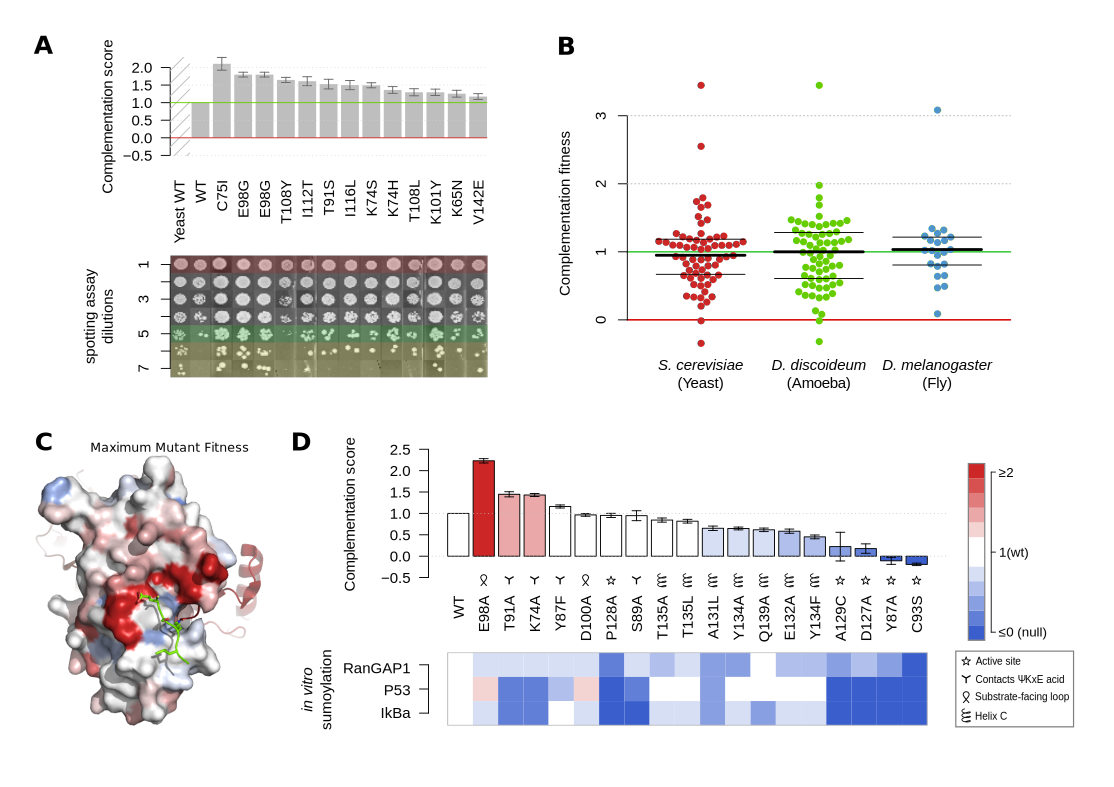
\includegraphics[width=\textwidth]{img/hyperactive.pdf}
	\caption{Hyperactive complementation in UBE2I. A) Variants scoring higher than the wildtype controls show stronger growth in manual complementation spotting assays and resemble the WT yeast. B) Distribution of scores for changes to residues naturally occurring in yeast, amoeba and fly are not significantly different from each other. C) Maximum mutant score mapped to amino acid positions on UBE2I structure. Hyperactive mutations are clustered at the substrate recognition site. D) \textit{In vitro} sumoylation assays performed by Bernier-Villamor~\etal~\cite{bernier-villamor_structural_2002} in comparison to complementation fitness scores.}
	\label{fig:hyperactive}
\end{figure}


As Figure~\ref{hyperactive}D shows, substrate specificity does not paint a complete picture of the mechanisms potentially underlying hyperactive complementation. A particularly interesting exception can be observed at residues A15 and T108. Both residues harbor hyperactive mutations but do not face towards the substrate. Instead, they form part of the interface with the E3 SUMO ligase RanBP2, and flank a small cavity on UBE2I's surface into which RanBP2 inserts a phenylalanine residue upon binding~\cite{gareau_determinants_2012}. Changing either A15 or T108 into aromatic residues results in a large fitness increase (Figure~\ref{fig:pi-stack}). This may be the result from the emergence of a $\pi$-stack interaction that strengthens E2-E3 binding.

\begin{figure}[h!]
	\centering
	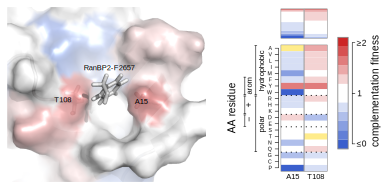
\includegraphics[width=\textwidth]{img/pi-stack.pdf}
	\caption{Potential de-novo pi-stack interaction between UBE2I and the E3 RanBP2}
	\label{fig:pi-stack}
\end{figure}

It is unclear how to interpret the effect of mutations that enhance growth in the yeast complementation assay. If fitness measured in the assay is directly proportional to fitness in the real biological context, then these enhancing mutations would be beneficial. However one can also imagine an alternative scenario in which activity-enhancing mutations are deleterious in the real biological context. To objectively distinguish between these possibilities, we collaborated with Jesse Bloom to employ a method he recently published that leverages likelihood-based phylogenetics to quantitatively compare how well different experimental measurements represent actual evolutionary constraints in nature~\cite{bloom_experimentally_2014,bloom_identification_2017}. We compared three models relating the experimental fitness to the evolutionary preference for a mutated amino-acid sequence: (a) the evolutionary preference was directly proportional to the untransformed experimental fitness; (b) the preference had a ceiling at the wildtype experimental fitness (values greater than 1 were set to 1); or (c) the preference was set to the reciprocal of fitness for mutations with greater-than-wildtype scores, corresponding to a deleterious effect of enhancing mutations. Dr. Bloom kindly provided the phydms software~\cite{bloom_identification_2017} to test which of these three approaches best described the evolutionary constraint on a set of naturally occurring UBE2I homologs, using fitness scores that excluded conservation features from the regularization process, to avoid the circularity of using natural sequence data when deriving the scores. As shown in Table~\ref{tab:phydms}, the best fit is achieved using the model that assumes that enhancing mutations are deleterious. This result provides objective support for the idea that mutations that enhance activity above wildtype levels in the complementation assay are actually deleterious in a real biological context.

Based on these observations we reinterpreted cases of hyperactive complementation in our map as deleterious and repeated the imputation and regularization procedure. This lowered the cross-validation RMSD substantially from $0.33$ to $0.24$.

\begin{table}[h!]
	\centering
	\caption{Comparison of different models for the effects of hyperactivating mutations. AIC: Akaike Information Criterion\newline}
	\begin{tabular}{l l}
Model & $\Delta$AIC relative to best model\\ \hline\hline
Penalize hyperactive mutations & 0\\
Cap score of hyperactive mutations at wildtype level & 27.7\\
Hyperactive mutations as beneficial	& 60.6	
	\end{tabular}
	\label{tab:phydms}
\end{table}



\subsubsection{Intragenic epistasis and compensatory mutations}

Full-length UBE2I clones generated for DMS-BarSEQ analysis often encoded more than one amino acid change. Multi-mutant clones offer the opportunity to search for intragenic genetic interactions. Genetic interaction is defined when a combination of mutations yields an unexpected phenotypic effect, so that identifying genetic interactions requires that we model the phenotype expected from a combination of mutations, given the single-mutant effects.  Here we used a previously-described multiplicative model 20,21 in which genetic interaction is measured as $\varepsilon_{ij} = f_i \cdot f_j - f_{ij}$, where $f_i$ and $f_j$ represent single mutant fitness and fij represents double mutant fitness scores. Most double mutants (71\%) did not show a significant deviation from $\varepsilon_{ij} = 0$ under this model, while 328 position pairs did show significant genetic interaction (Figure~\ref{fig:epsistasis}, see Methods). Of particular interest are compensatory interactions, i.e. cases where a double mutation is more fit than either of the component single mutations.  Where compensatory residues are proximal in the protein structure, the combination of two mutant residues may be able to re-establish a physical interaction that was lost in each of the single mutants. Although the majority of genetically interacting sites were not proximal in the structure (Figure~\ref{fig:epsistasis}B), there were interesting exceptions. For example, the I4T-P69S double mutant appears to exhibit compensatory behaviour: In the wild type structure, the van-der-Waals radii of the two residues are in direct contact (Figure~\ref{fig:epsistasis}C). Either mutation alone would be expected to destabilize the hydrophobic interaction between isoleucine and proline.  However, In the double mutant, hydroxyl groups on the two residues could adopt a hydrogen bond that re-establishes interaction and re-stabilizes the fold (Figure~\ref{fig:epsistasis}D).

\begin{figure}[h!]
	\centering
	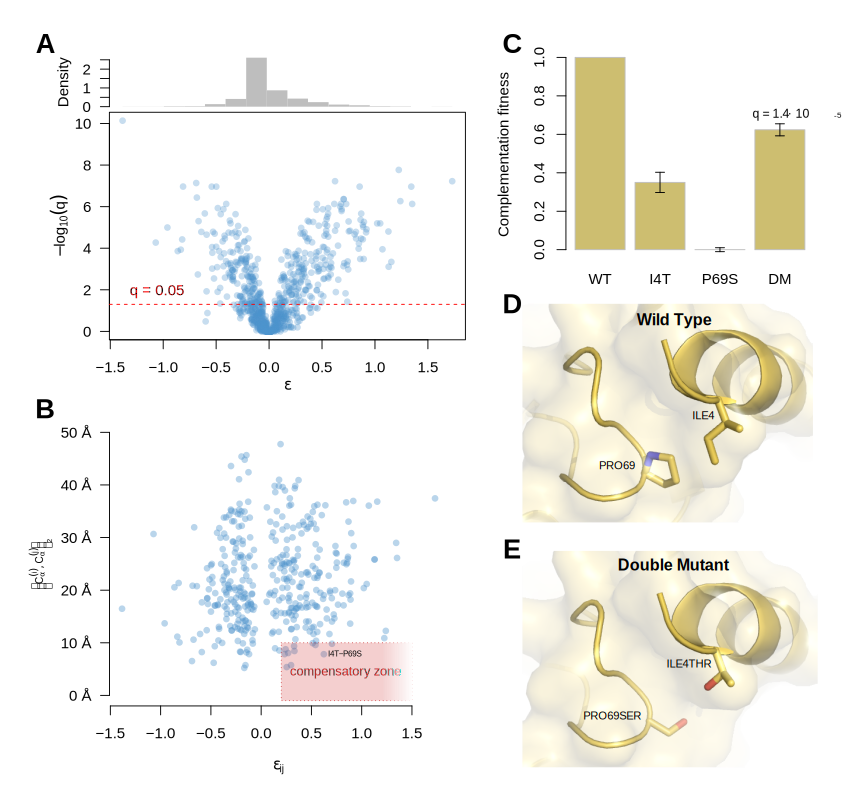
\includegraphics[width=\textwidth]{img/epistasis.pdf}
	\caption{Epistasis}
	\label{fig:epsistasis}
\end{figure}


\subsection{A functional map for SUMO1}

Using the DMS-TileSeq version of the framework established in the previous chapter we also created a complete functional map for SUMO1 (Figure~\ref{fig:sumo-map}A). The most immediately apparent feature of the SUMO1 map was the strong enrichment for neutral substitutions within the first 20 amino acid positions, which is consistent both with the low level of evolutionary conservation for this region and its annotation as a disordered region. The last four amino acid positions appeared similarly insensitive to mutation, consistent with the cleavage of this region by SENP proteases during SUMO maturation. By contrast, other residue positions were strongly sensitive to mutation, including many inward-facing residues that are apparently constrained to be hydrophobic. As expected, the C-terminal diglycine, directly preceeding the last four cleaved residues, is also very sensitive to mutation, as it is required for the covalent binding of SUMO to the E1, the E2 and to the sumoylation target protein.Interestingly, except for the C-terminal diglycine, the residues that directly touch the E2 during covalent binding are not as sensitive (Figure\ref{fig:sumo-map}B). This may be due to  SUMO being force-fed to the E2 by the E1 activating complex and the thioester bond it forms with the E2's cystein \#93 is all that is needed to maintain the complex. By contrast, residues in the interface for non-covalent E2 binding are much more sensitive (Figure\ref{fig:sumo-map}C). Especially leucine \#80 and methionine \#82 appear to be important

Other strongly constrained residues are core members of interaction interfaces. These include the central phenylalanine 36 in the SUMO recognition motif (SRM) interface; glycine 68, which forms the apex of a tight turn within the interface with de-sumoylation enzymes, as well as the E1 and E2 proteins; and leucine 80, which is part of the interface with non-covalently bound E2. 

\begin{figure}[h!]
	\centering
	\includegraphics[width=\textwidth]{img/sumo-map.pdf}
	\caption{Functional map of SUMO1}
	\label{fig:sumo-map}
\end{figure}

The proximity and orientation of aspartate \#73 and lysine \#48 suggests that they are able to form a salt bridge with one another.  The importance of each residue according to the DMS map supports a model in which this salt bridge is important for SUMO folding and/or stability. Interestingly, substituting aspartate for methionine \#59, which points towards lysine \#48 from an angle similar to that of aspartate \#73, enhances the complementation fitness of SUMO1 beyond wild type levels.  This further underlines the potential importance of a polar interaction involving lysine \#48 (Figure~\ref{fig:saltbridge}).

\begin{figure}[h!]
	\centering
	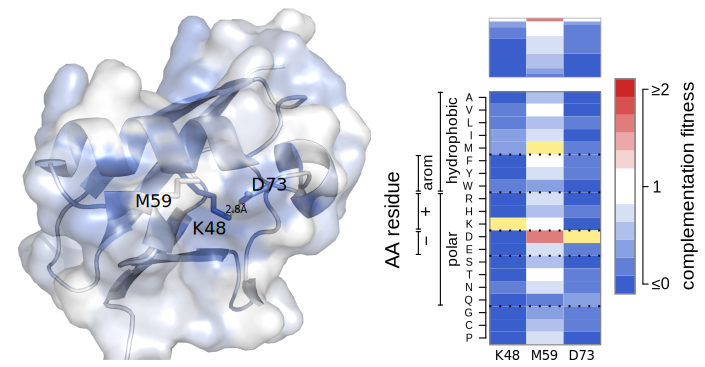
\includegraphics[width=\textwidth]{img/saltbridge.pdf}
	\caption{A salt bridge within SUMO1 between Asp73 and Lys38 appears important for stability. Met59Asp may increase stability even further.}
	\label{fig:saltbridge}
\end{figure}


% As was shown above for UBE2I, phylogenetic analysis of SUMO1 similarly showed that adaptive mutations with ability to complement yeast better than wild-type are likely deleterious in humans. We therefore transformed fitness scores so that such adaptive mutations are considered to be deleterious (see Methods).  However, because adaptive substitutions may provide interesting clues about differences between yeast and human cellular contexts, we provide both transformed (Figure 5) and untransformed versions of each map.




\subsection{Functional maps of three human disease genes}

Having established and evaluated our Deep Mutational Scanning framework on two members of the sumoylation pathway, we aimed to create maps for a diverse set of genes that have been associated with disease with varying degrees of confidence. While  heterozygous null mutations in SUMO1 have previously been associated with cleft palate, we wished to create maps that could be tested in the context of variant classification in terms of disease. Based on the availability of robust complementation assays, we applied DMS-TileSeq to the following protein targets: Thiamine Pyrophosphokinase 1 (TPK1), associated with vitamin B1 metabolism dysfunction; Neuronal Calcium Sensor 1 (NCS1), which has been implicated in autism based on a single \textit{de novo} mutation;  and CALM1, CALM2 and CALM3 associated with heart conditions long-QT syndrome and catecholaminergic polymorphic ventricular tachycardia. Although the three calmodulin genes differ in nucleotide sequence, each encodes the same polypeptide sequence. Thus, we performed a deep mutational scan only for CALM1, which enabled us to also map missense variant effects in CALM2 and CALM3. In each case, we used the TileSEQ approach coupled with complementation to generate a map of missense variant functions. 

As was shown above for UBE2I, phylogenetic analysis of SUMO1 similarly showed that variants with ability to complement yeast better than wild-type are likely deleterious in humans. We therefore transformed fitness scores so that such adaptive mutations are considered to be deleterious \todo{expand on this}. The transformed disease gene maps can be seen in Figures \ref{fig:tpk1-map} and \ref{fig:calm+ncs1-maps}).  However, because adaptive substitutions may provide interesting clues about differences between yeast and human cellular contexts, we also provide untransformed versions of each map (see Appendix).

%%FIGURE: Map for TPK1/NCS1/CALM1


\subsubsection{A thiamine pyrophosphokinase map reflects a recessive phenotype}

Thiamine pyrophosphokinase (TPK1) is a protein that forms a dimer to perform its biochemical function. Its substrate, thiamine diphosphate, is bound within two active sites formed by the dimerization interface\cite{timm_crystal_2001}. That is, each monomer contributes half of the residues making up each of the two active sites.  Each monomer in turn is made up of an N-terminal globular domain and a C-terminal $\beta$-sandwich domain (Figure~\ref{fig:tpk1_structure}A). The residues most sensitive to mutation in the protein make up the hydrophobic cores of the two domains: L21, V22, W36, G48, Y53, P65, G70, Y83, L108, I122, T124, and G127 for the N-terminal domain; and L161, G168, G199, L200, V227, V229, L236, and W237 for the C-terminal domain (Figure~\ref{fig:tpk1_structure}B). As might have been expected, mutation-sensitive residues include those closely involved in forming the active sites: D46, G70, D71, D73, D100, and K103 in the N-terminal half of the active site , contacting the diphosphate portion of the substrate (Figure~\ref{fig:tpk1_structure}C). In the C-terminal half of the active site, K203, L209, G212, L214, S216, T217, and N219 show similar sensitivity. Interestingly, the tryptophan residue at position 202 appears to be insensitive to mutation despite its close and extensive contact with the thiamine ligand. By contrast, a neighbouring lysine at position 201 is surprisingly sensitive suggesting potential importance in coordinating the ligand.  The remainder of the dimerization interface also features a number of sensitive residues, such as M136, G184, V188, G189 and G211. Finally, residues 1-12, which form a $\beta$-strand anchoring the N-terminal domain back to the C-terminal domain were also found to be sensitive.

\begin{landscape}
\begin{figure}[h!]
	\centering
	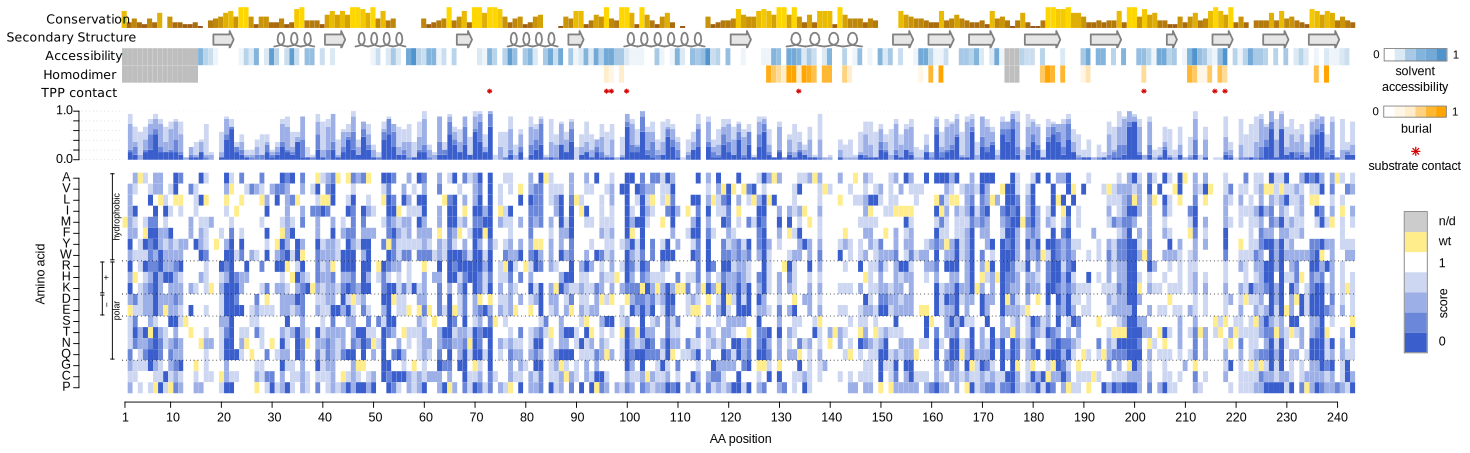
\includegraphics[width=9in]{img/tpk1-map.pdf}
	\caption{Functional map of Thiamine pyrophosphokinase 1 (TPK1). From top to bottom: Position-wise evolutionary conservation (AMAS); Secondary structure; Relative solvent accessibililty; Relative burial in homodimerization interface; Contacts with Thiamine diphosphate; Summary track showing the shares of amino acid changes resulting in varying degrees of fitness effects; Detailed heatmap showing individual amino acid change effects.}
	\label{fig:tpk1_structure}
\end{figure}
\end{landscape}

\begin{figure}[h!]
	\centering
	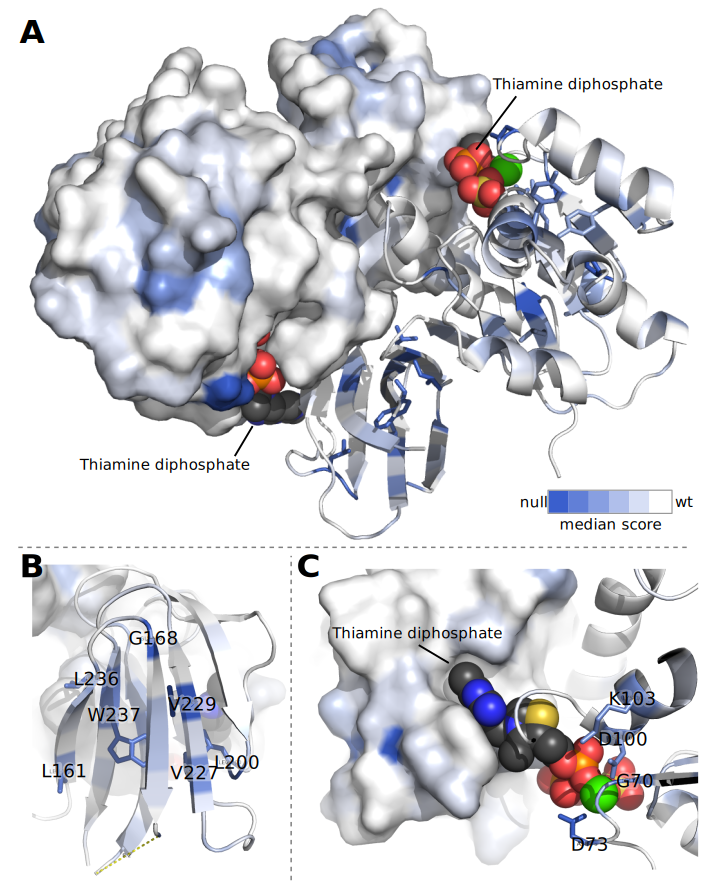
\includegraphics[width=.8\textwidth]{img/tpk1_structure.pdf}
	\caption{Thiamine pyrophosphokinase 1 colored by median complementation score. A) TPK1 homodimer structure showing one monomer as surface model, the other monomer as cartoon model. B) Hydrophobic residues facing the inside of the C-terminal $\beta$-sandwich domain are sensitive to mutation. C) Active site residues in contact with the substrate are sensitive to mutation.}
	\label{fig:tpk1-map}
\end{figure}


\subsubsection{The two calcium sensors NCS1 and Calmodulin show different profiles}

Calmodulin (CALM1/2/3) and the Neuronal Calcium Sensor protein (NCS1) are homologs (E-value $4 \cdot 10^{-5}$ when searched against the human proteome~\cite{altschul_basic_1990,the_uniprot_consortium_uniprot:_2015}) with 24\% sequence identity and 48.5\% similarity~\cite{rice_emboss:_2000}. However, they display different impact patterns despite their similar domain structure and similar molecular roles as calcium sensing proteins. Both are comprised of four Calcium-binding EF-hands, with NCS1 containing additional sequences upstream and downstream of the four hands. A comparison of previously published NMR structures reveals that the overall folds of the two proteins differ substantially~\cite{sarhan_crystallographic_2012,heidarsson_c-terminal_2012}. Calmodulin features a long central helix that separates two globular domains, called the N-lobe and the C-lobe, each comprised of two EF hands. A hydrophobic pocket serving as a binding interface for interacting proteins is nested within the C-terminal domain. NCS1, by contrast, forms a single shell-like shape, centered around a large hydrophobic crevice. This crevice acts as a binding interface for interacting proteins. Thus, the divergent DMS profiles we observed for CALM1/2/3 and NCS1 are consistent with these substantial structural differences.

The Neuronal Calcium Sensor NCS1 displays the greatest sensitivity to mutation within the N-terminal region containing the myristoylation site.  This myristoylation site is essential for anchoring NCS1 into the plasma membrane. One other residue that stands out is the tryptophan at position 30, which results in complete loss of function when replaced with any other amino acid. Like most other sensitive residues W30 is found among those contributing to the hydrophobic crevice acting as an interaction interface. Other cases include F55, F56, A104, M121, I152, and A182. An interesting observation can be made with respect to the two helices that separate the two N-terminal EF hands from the two C-terminal EF hands. A kink between the two helices brings them into an angle that allows a the globular shape of the overall protein to form. Without this kink it is conceivable that NCS1's fold would much more resemble that of Calmodulin. A glycine residue (G95) is likely responsible for forming that kink due to its helix breaking properties. This residue is also found to be quite sensitive to mutation.

Within Calmodulin, the regions most sensitive to mutation are: 1) the hydrophobic cores of the two globular domains; 2) interfacial residues for protein-protein interactions, and 3) a subset of the negatively charged residues in EF hands that contact Ca$^{2+}$ ions. Within the hydrophobic cores of the two lobes, five mutually interacting phenylalanine residues at positions 17, 69, 90, 93, and 142 stand out in particular, as all of them are found in the top 9 most sensitive residues on the map. Within the interaction interface, the residues D85, A89, F93, M100, L106, V109, L113, G114, L117, M125, V137, F142, M145, M146 are the most strongly sensitive to mutation. Regarding the four Calcium-binding EF-hand loops, we found it interesting that only a subset of the negatively-charged residues contacting Ca$^{2+}$ are even moderately sensitive. Within EF1, only D25 appears to be important, in EF2 only N61, in EF3 only D94 and D96, and in EF4 only D130 and D134. Overall, the EF3/4 in the C-lobe also appear to be more important than their N-lobe counterparts. This is in agreement with previous observations made by Sarhan and colleagues~\cite{sarhan_crystallographic_2012}, who described the C-lobe as the primary sensory mechanism. A number of unexplained sensitivities exist as well: Arginines at positions 54 and 91 show strong phenotypes despite extending from seemingly unused surfaces of the protein, offering the possibility that these residues are functionally relevant sites of interaction or modification.


\begin{landscape}
\begin{figure}[h!]
	\centering
	\includegraphics[width=9in]{img/calm+ncs1-maps.pdf}
	\caption{Functional map of Thiamine pyrophosphokinase 1 (TPK1). From top to bottom: Position-wise evolutionary conservation (AMAS); Secondary structure; Relative solvent accessibililty; Relative burial in homodimerization interface; Contacts with Thiamine diphosphate; Summary track showing the shares of amino acid changes resulting in varying degrees of fitness effects; Detailed heatmap showing individual amino acid change effects.}
	\label{fig:calm+ncs1-maps}
\end{figure}
\end{landscape}


\subsubsection{Functional maps recapitulate known disease cases}

To validate the utility of our maps in the context of human disease, we extracted known disease-associated variants from Clinvar~\cite{landrum_clinvar:_2016}, as well as rare and common polymorphisms observed independent of disease from GnomAD~\cite{lek_analysis_2016}, and somatic variants previously observed in tumors from COSMIC~\cite{forbes_cosmic:_2001}. 

For TPK1, a large number of very rare variants (minor allele frequency or $\text{MAF} < 10^{-6}$) is known from GnomAD. At first look, it appears the majority of these variants are shown to be deleterious (Figure~\ref{fig:tpk1_diploid}). This seems unlikely, given that Thiamine Metabolism Dysfunction Syndrome, reported to be caused by mutations in this gene, is a very severe disease to which patients succumb in childhood~\cite{mayr_thiamine_2011}., and that GnomAD attempts to filter out subjects with severe pediatric disease. However, the disease is also known to follow a recessive inheritance pattern, with only homozygous or compound heterozygous individuals being affected. We thus used phased sequence data from the 1000 Genomes Project~\cite{the_1000_genomes_project_consortium_global_2015} to determine the diploid genotypes in the TPK1 locus for all listed individuals and based our phenotype predictions based on the maximum fitness score of either allele. This improved prediction performance markedly, leading to complete separation between disease and non-disease genotypes. Both PROVEAN and PolyPhen-2 were also able to perfectly separate the two groups (Figure~\ref{fig:tpk1_diploid}B), so that additional compound heterozygotes with known disease status will be required to determine whether this DMS map is more useful than computational methods for classifying pathogenic TPK1 variants. 

\begin{figure}[h!]
	\centering
	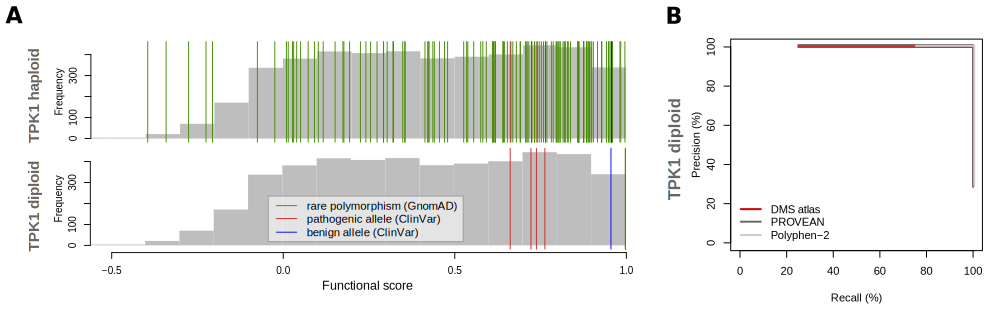
\includegraphics[width=\textwidth]{img/diploid.pdf}
	\caption{TPK1 variants}
	\label{fig:tpk1_diploid}
\end{figure}


While NCS1 does not have any entries in ClinVar, a previous publication identified the variant R102Q as a \textit{de novo} variant in a single patient with autism spectrum disorder~\cite{handley_structural_2010}. While the variant did not affect overall protein folding and localization, the authors did observe that the dynamics of cytosol-membrane cycling were altered. Our complementation map did not show any functional impact for this variant.

As for NCS1, no disease-associated missense alleles are known for UBE2I and SUMO1 in ClinVar. However, a number of somatic mutations for all three genes have been observed in cancer according to COSMIC. While these can be expected to passenger mutations, one may still hypothesize that somatic variants are likely not subject to the same selection pressures as germline variants, as interference with developmental processes is not necessarily detrimental to a tumour. We thus tested whether germline polymorphisms in these three genes were enriched for being functional compared to their somatic counterparts in our maps. Indeed, we observed a significant difference between the two sets (Wilcoxon $P = 2.6 \cdot 10^{-5}$) (Figure~\ref{fig:calm_disease}C).

Finally, we examined our functional map of Calmodulin and found that it was able to distinguish disease variants from non-disease variants very well (Figure~\ref{fig:calm_disease}A). In contrast to TPK1, the Calmodulin map did not need to be corrected for diploid genotypes, as previously reported disease variants have been described as following a dominant inheritance pattern~\cite{crotti_calmodulin_2013}. A precision-recall (PRC) plot reveals a superior performance (AUC = 0.74) compared to PROVEAN (AUC = 0.47) and PolyPhen-2 (AUC = 0.47).  

\begin{figure}[h!]
	\centering
	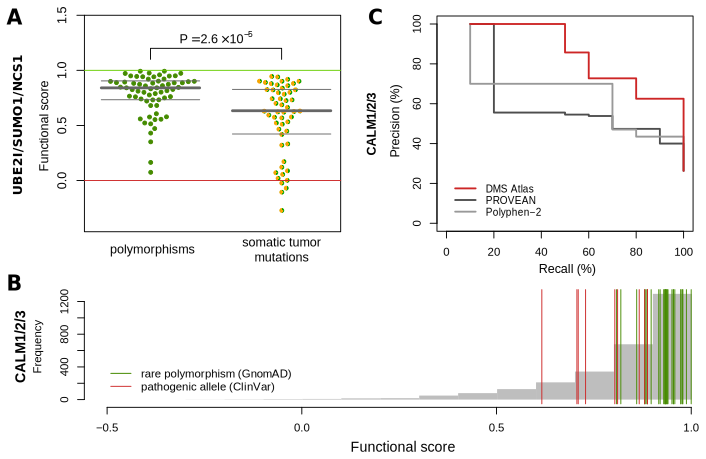
\includegraphics[width=\textwidth]{img/calm_disease.pdf}
	\caption{Calmodulin variants}
	\label{fig:calm_disease}
\end{figure}


To further put our map to the test in a clinical scenario we inquired with Invitae, a company offering gene panel sequencing services for Long QT syndrome, including CALM1/2/3. In a blind test, we requested a list of Calmodulin variants they observed in patients but were unable to classify. After calibrating our map with respect to the above ClinVar and GnomAD datasets, we classified these 10 new variants (Table~\ref{tab:invitae}). Two were classified as damaging, six as benign, and two were too close to the threshold to be called either. In the next phase, Invitae revealed the associated patient cardiovascular phenotypes. Five out of the six patients with benign predictions were revealed to be healthy, while both patients with damaging predictions did show a positive phenotype. The two uncertain cases were revealed to be affected as well. A Mann-Whitney-U test showed these results to be statistically significant (P = 0.008).

% \begin{table}
% 	\centering
% 	\caption{}
% 	\begin{tabular}{l l l}
		
% 	\end{tabular}
% 	\label{tab:invitae}
% \end{table}

\section{Discussion}

\section{Methods}





\chapter{Conclusion}

\section{Summary}

Here we have presented a complete framework for the construction of comprehensive, high-fidelity functional maps. We have demonstrated two versions of this framework: DMS-BarSeq, a barcode-based approach that allows for high-confidence measurement of individual clones including double- and higher-order multi-mutants; and DMS-TileSeq, a fast and efficient framework that generalizes fitness effects over many different clones sharing variants of interest. Both versions use a new mutagenesis protocol, POPCode, which thanks to its accompanying webtool makes it easer than before to generate variant libraries covering the complete space of amino acid changes. At its core, the framework relies on a functional complementation assay in yeast, which can measure the overall effect of variants on protein function and has been shown to be highly predictive of variant pathogenicity in humans, outperforming common \textit{in silico} methods, despite the $\sim$ 1 billion year divergence between the two organisms. 
The DMS analysis software developed here introduces novel advances to deep mutational scanning: (i) The degree of confidence behind each measurement is carefully assessed and recorded in order to help variant classification; and (ii) variants that were missing in the complementation library or measured with low confidence were supplemented using a RandomForest-based machine learning method, whose predictions were found to be surprisingly reliable. 

We have evaluated the technical features of the framework on the two sumoylation pathway members UBE2I and SUMO1. We found that the functional maps generated with our method were able to successfully recapitulate known features of the proteins' biology and biochemistry and even hint at novel features that warrant further investigation. We found a large number genetic interactions between variants in UBE2I, some of which may be due to direct compensatory relationships of amino acid replacements. Most interactions however were found to involve residue pairs separated by larger physical distances.

Having validated the framework, we demonstrated its power to detect pathogenic variants in the disease genes \gene{TPK1}, \gene{NCS1}, \gene{CALM1}, \gene{CALM2} and \gene{CALM3}.  
We found that our Calmodulin map excelled at distinguishing disease-associated variants from benign polymorphisms and greatly outperformed the common prediction algorithms PolyPhen-2 and PROVEAN. We subsequently applied our functional map for \gene{CALM1}, \gene{CALM2} and \gene{CALM3} to classify VUS observed in patients during gene panel sequencing and found our predictions to be closely matching patient indications.

\subsubsection{Limitations of the DMS framework}
Despite these successes, there are a number of limitations the current form of our DMS framework. A fairly simple problem is the current restriction to scan relatively short genes. This is due to three reasons: (1) Longer genes would require a re-formulation of the mutagenesis protocol, as the number of mutations introduced per clone can be expected to increase linearly with gene length. This would need to be addressed by varying the concentration of mutant oligos in the amplification step. This could be tested systematically for templates of different lengths to determine the exact relationship between the factors involved. The results can then be added to the POPCode oligo design software to automatically report the most suitable protocol for each case to the experimenter.
(2) Variant clone pools for longer genes must be kept in larger volumes at all times to avoid bottlenecking the complexity of the pools.
(3) Finally, larger libraries also require more sequencing reads to cover all variants at adequate depth. Thus they either require the use of higher-throughput equipment or would have to be processed in batches. 
A relatively easy solution to all three problems would be subdivide longer genes into sections that would be scanned separately from each other, although this would be more time consuming and costly.

A more difficult problem is that currently, the number of genes amenable to functional complementation in yeast is very limited. Song Sun and other members of the Roth lab have previously determined that only 60 human disease genes can currently been examined using this assay~\cite{sun_extended_2016}. In addition, we found that some of these genes suffer from mapping quality issues. We observed this in the \gene{NCS1} map, which was of lower quality compared to other genes due to its relatively weak wildtype complementation fitness resulting in a less favourable signal-to-noise ratio. However it is possible that these assays might be improved by using different yeast strains with different backgrounds or by using different growth conditions.
Moreover, as mentioned in section~\ref{ch2discussion} of the previous chapter, we have determined that 57\% of disase genes could be assayed using DMS variants based on Y2H or human cell lines instead, as will be discussed in further detail in the next section.


\section{Outlook}

\subsection{Using DMS data in a clinical context}
%DMS in clinical contexts
As introduced in chapter 1, a major motivation factor behind the development of our framework is to address the growing problem of variants of uncertain significance observed in the clinic. While our results show that functional maps as produced by our framework can be helpful in the effort of VUS reclassification, a single line of evidence is not usually sufficient. Even though the ACMG considers functional assays among the strongest classification criteria, they require at least one additional criterium of moderate strength, such as enrichment in cases over controls, or negligible allele frequency in the general population~\cite{richards_standards_2015}. While most of the information informing the required criteria cannot be generated \textit{en masse}, other information, such as allele frequencies in the general population are available from the 1000 genomes project~\cite{the_1000_genomes_project_consortium_global_2015} and the genome and exome aggregation database (GnomAD)~\cite{lek_analysis_2016}. Thus an important goal for the future would be the construction of a public database with an underlying automatic data integration and classification system, that obtains information from available sources and automatically applies the ACMG's recommended decision-making process towards variant classification. Classification results should be presented transparently, revealing the individual underlying evidence, confidence levels and reasoning structure. 

However, the commitment towards the construction of a resource is only warranted if its primary source of information, functional maps generated using Deep Mutational Scanning can continue to be provided. The Roth Lab is planning to continue building functional maps of disease genes and to expand the list of genes amenable to deep mutational scanning. A shortlist of $\sim$100 genes is planned to be addressed in the coming years. However, this undertaking is a costly one. Per 500 amino acid positions scanned, approximately \$5500 need to be spent on consumables, primarily for sequencing and oligos for POPCode mutagenesis. Assuming 6 genes being scanned in parallel, approximately 45 full-time employee hours need to be invested per gene. Ultimately, this undertaking cannot be stemmed by one lab alone and will require outreach to other groups. As shown in chapter~1 section~\ref{dmsIntro} a fair amount of groups are already performing deep mutational scans, who may be interested in collaboration. As a first step, the Roth and Fowler labs are already planning on collaborating with respect to mapping a number of heart-disease associated genes.

\subsection{Adaptation and extentions to DMS technology}
\subsubsection{DMS in human cell lines}
As mentioned above, an important future direction is the adaptation of the deep mutational scanning framework toward directly using human cell lines in the competition assays. Recent genome-wide CRISPR screens have revealed a sizable number of genes with growth phenotypes in different human cell lines~\cite{hart_high-resolution_2015,blomen_gene_2015,wang_genetic_2014}. While a number of DMS efforts have already been performed using human cells~\cite{forsyth_deep_2013,wagenaar_resistance_2014,doud_site-specific_2015,majithia_prospective_2016}, the underlying assays were not generalizable, for example, the most recent effort by Majithia and colleagues~\cite{majithia_prospective_2016} for PPAR$\gamma$ was only possible due to the fortuitous circumstances of having found a surface marker whose expression level directly reflects PPARG$\gamma$ activity. 
Atina Cote in the Roth Lab is currently working on establishing a generalizable growth-based assay using CRISPR in human cell lines. 
%previous work: PPARG
%atina's CRISPR lines
%fowler's stability assay

\subsubsection{Screening of other functional elements}
Another important future direction is to expand the capability of Deep Mutational Scanning to enable the assaying of variants outside of protein-coding regions of the genome. However, since the space of the human genome is simply too large to be tested in its entirety the logical choice is to concentrate on elements most likely to be functionally relevent, such as splice sites, promoters, or transcription factor binding sites.
Hanane Ennajdaoui in the Roth Lab is currently working on adapting our DMS framework to scan intron boundaries.
%spliceDMS

\subsection{Other uses of DMS functional map data}

\subsubsection{Screening for viral suppressors}
Deep Mutational Scanning has many other potential uses beyond disease variant classification. As we have demonstrated in chapter 3 for UBE2I, the method helps sheds light on the biophysical mechanisms underlying the function of a gene. We have also shown that using a combination of Y2H and complementation, DMS can point to potential new protein interaction interfaces. 

UBE2I is known to be directly targeted by many viruses, such as HIV, and EBV,  through specific protein-protein interactions to subvert host defenses~\cite{varadaraj_sumo_2014}. Using Y2H as the selection assay in our DMS framework and using our exising functional map of UBE2I as a reference, it would be possible to scan for variants that specifically disrupt interactions with viral proteins while not affecting overall UBE2I function. At the same time, this approach could help finding the specific interface for the interactions in question and could inform future drug development.

\begin{figure}[h!]
	\centering
	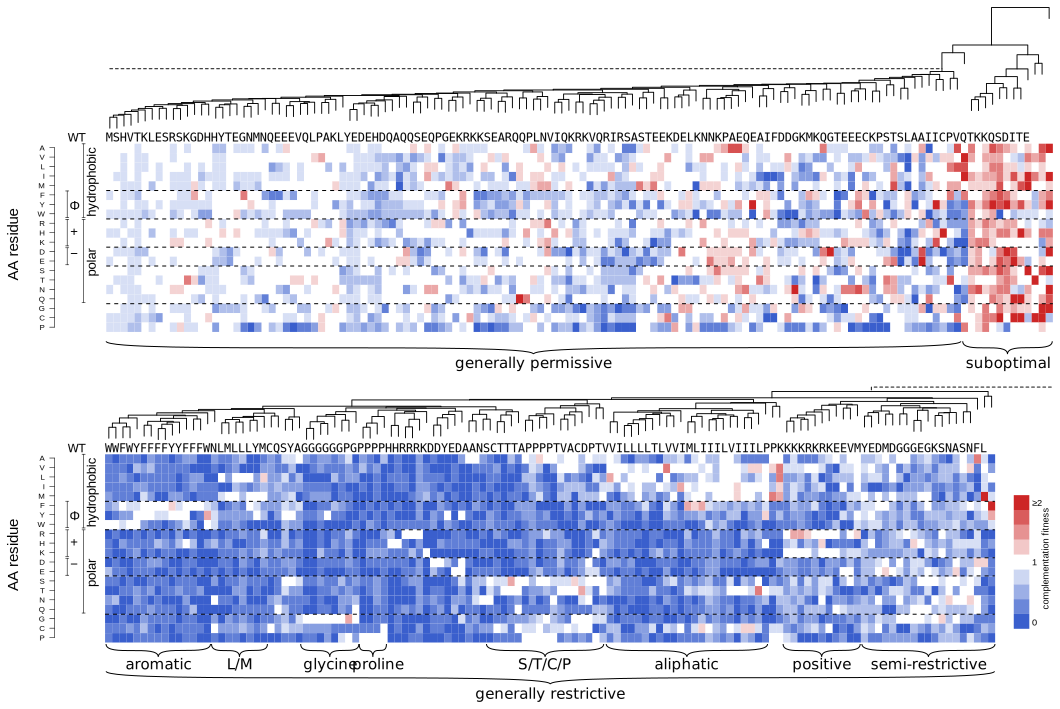
\includegraphics[width=\textwidth]{img/clustering.pdf}
	\caption{Hierarchical clustering of amino acid positions in UBE2I and SUMO1.}
	\label{fig:clustering}
\end{figure}

\subsubsection{Advances in computational prediction of disease variants}
As the number of functional maps produced via DMS grows, so does the its value as training data for \textit{in silico} prediction methods. While currently the number of genes scanned is not yet representative enough to cover the functional diversity of the proteome. However, Yingzhou Wu in the Roth Lab has already begun to explore its potential value for extrapolation. In an initial experiment, he was able to show that a machine learing method trained on the functional data obtainer for UBE2I was able to make better predictions towards the the effects mutations in SUMO1 than if trained on the data set underlying PolyPhen-2 (HumDiv). Thus, with each new functional map added to our variant atlas, computational predicion method have the potential to become more powerful.
%  -> FUNSUM

\subsubsection{Functional classification of amino acid positions}
The same wealth of functional data that may serve as training data for future computational prediction methods may also help us learn more about the set of roles played by different residues within proteins. In an initial experiment I have generated a hierarchical cluster map across postions in UBE2I and SUMO1 (Figure~\ref{fig:clustering}). The clustering hints at distinct functional classes occupied by different positions. There are three broad groups: (1) Positions that are generally unrestricted and can be occupied by almost any amino acid; (2) Positions that are generally constrained to a certain small number of amino acids and; (3) Positions that show result in hyperactivity for many possible amino acids. Within these groups there are a number of subclusters visible. For example, within group two, certain positons only tolerate alphatic residues, while others only tolerate aromatic residues. Evolution only samples a subset of the possible amino acids at a given position. By growing the set of proteins with complete functional maps we can potentially collect a catalog of possible functional `archetypes' for positions within proteins. Using multiple alignments we can then make predictions as to the archetype of any given position.
% -> functional classes


%% This adds a line for the Bibliography in the Table of Contents.
\addcontentsline{toc}{chapter}{Bibliography}
\bibliographystyle{unsrt}
{\small
\bibliography{thesis}
}
\end{document}
